%pdflatex-../thesis.tex
% vim:spell spelllang=en_us

There are common routines in cloud data center administration and these routines are repeating very frequently. For example simple workflow for virtual machine creation can involve:
\begin{itemize}
	\item clone image with prepared operating system
	\item log into hypervisor console and create \Ac{VM} definition
	\item deploy virtual machine 
	\item configure firewall and router 
	\item configure vswitch or attach virtual machine into bridge
	\item set up network interfaces in \Ac{VM}
	\item set root's password and add authorized keys
	\item update monitoring definition
\end{itemize}

There can be dozens of task similar to mentioned above and it can take negligible amount of time. These task are usually very simple and all necessary information can be generated automatically or loaded from an information system. It is very favorable to perform these task automatically because it does not need any assistance of human and automated solution is much more faster and strictly deterministic.

Orchestration is automated management of services and resources performed according to predefined procedure. An inteligence is implemented into orchestrator so it can make desicions and execute actions without an interaction with human. Orchestrator acts autonomously according to configurated parameters in contrast to remote control interface which only perfroms requested actions.

It is necessary to use orchestration for every cloud solution because it is not possible to cope with manual configuration and management of many cooperating services and resources. Rapid provisioning with minimal management effort is required in cloud computing definition mentioned in the beginning of this chapter and it can not be accomplished withou orchestration.

% configuration management
There exists actually one more step between completely manual management and orchestration and it defined by using configration management. Configuration management solution is used for uniform management of configuration and executing repetitive task. It is possible to develop own solution or use any software available. For example Ansible, Puppet or SaltStack are well know open-source softwares. Configuration management software can be instegrated into orchestrator and used as a interlayer between orchestrator and performed actions.
Ansible is used for virtual machine configuration used in practical part of this thesis as well as for installation and configuration of OpenNebule IaaS cloud. It creates cloud environemnt with defined parameters and prepare initial configuration so it significantly shorten time required for installation and also eliminates configuration mistakes.  

\subsection{OpenNebula}
OpenNebula is open source cloud OS capable of building IaaS solution, so it is technically an orchestrator. \cite{opennebula} However it is not only an orchestrator but complete solution for datacenter orchestration capable to build \Ac{IaaS}. It was initially created as an research project in 2005 and the first public release was in 2008. It is currently developed by the community in cooperation with OpenNebula Systems.

It is completely platform agnostics so mayor virtualization techniques can be used. \Ac{KVM}, XEN and VMware is supported at current time but it is possible to develop modules for other virtualization platforms. There is for example driver OneLXC developed by China Mobile and this driver brings support for \Ac{LXC} hosts and containers.

Project architecture is module and can be modified according to system requirements. There is one node called frontend which is responsible for orchestration and other nodes are used as computing nodes, i. e. hypervisors. It is not required to dedicated separate hardware node for frontend because it can be deployed on physical server together with computing node. However it is recommended to deployed frontend as a virtual machine in \Ac{HA} since it is more flexible and robust. Sample physical infrastructure is depicted in figure \ref{img:opennebula-arch}.

\begin{figure}[htb]
	\begin{center}
	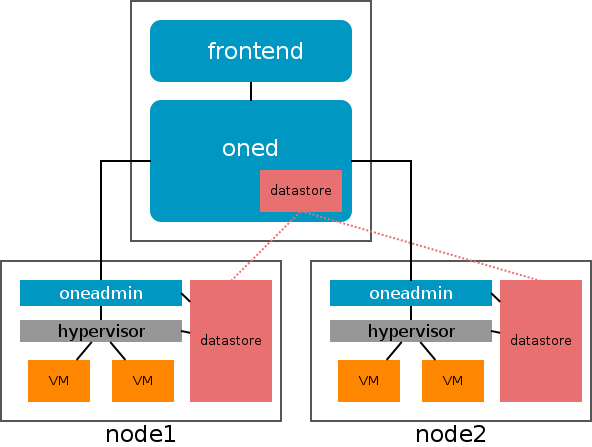
\includegraphics[width=0.8\textwidth]{opennebula-arch.png}
	\end{center}
	\caption{OpenNebula architecture}
	\label{img:opennebula-arch}
\end{figure}

Frontend acts orchestrator and uses additional modules to operate cloud infrastructure. There modules are universal to work with various underlying systems and each module must provide standardized interface for orchestrator. Modules and functions as defined in \cite{opennebula} are:
\begin{description}
	\item[Infrastructure and cloud drivers] enable access to infrastructure and cloud providers
	\item[Virtual machine manager] is used for managing \Ac{VM}s and executing action on them
	\item[Network manager] provide network configuration and management
	\item[Storage manager] supply storage for services and customers
	\item[Image manager] maintain library of \Ac{VM} images
	\item[Information manager] is collecting runtime information about physical infrastructure, \Ac{VM}s and other devices
	\item[Authentication and authorization] is used to authenticate users, store information about them, their permission and quotas
	\item[Accounting and auditing] gather information about resource usage and can be used to generate billing data
	\item[Federation manager] provide mechanism to access remote cloud providers
	\item[Scheduler] manages initial placement of new \Ac{VM}s according to scheduling policy
	\item[Administrative tools] provide interface for users and administrator to perform task on cloud system
	\item[Service manager] can work with group of interconnected \Ac{VM}s as with one service with defined requirements and deployment rules
\end{description}

% control
Orchestration is performed by frontend and remote tasks are executed at nodes using \Ac{SSH}. There is a single point of failure because frontend may go down so it is recommended to use \Ac{HA} solution and minimize possibility of frontend unavailability. However frontend failure does not affect running virtual machines since they stay online but monitoring will stop and it will not be possible to execute any action on virtual machines.o

% datastore
\subsubsection{Datastores}
Storage part of OpenNebula system is called datastore. It is abstraction of physical storage and is used to store persistent and non-persistent data. Persistent data are preserved during whole \Ac{VM} life cycle and non-persistent objects are restored to default state after virtual machine recreation. There are three types of datastore according to type and format of stored data:
\begin{description}
	\item[image] datastore is used to store images of non-running virtual machines
	\item[system] datastore hold images used of running \Ac{VM}s
	\item[files] datastore is used to save single files like kernels, contextualization data and files which are stored alone, meaning not as part of image
\end{description}

The image of virtual machine is cloned from image datatastore to system datatastore during deployment phase and then copied back after shutdown if image is persistent. Non-persistent images are not save back to system datastore so they can be directly destroyed. It is necessary to select technology for transfer to system datastore at nodes. There are options listed below, but it is possible create script for any other method original scripts are located at /var/lib/one/remotes/\{datastore,tm\}/.\footnote{It is necessary to run \Cmd{onehost sync} after changing any remote script at fronend.}
\begin{description}
	\item[shared] is filesystem directory and OpenNebula does not care about sharing technology, it just expects directory to be available on every node
	\item[ssh] can be used to transfer the images, it is always available but also vastly slow
	\item[vmfs] copies images using vmkfstools (VMware)
	\item[qcow] driver uses qemu-qcow to handle images
	\item[ceph] use ceph cluster to store images as \Ac{RBD}s
	\item[lvm] images are shared using clustered LVM
\end{description}

% networking
\subsubsection{Networking}
OpenNebula can assign virtual network to every running \Ac{VM} so networking driver is run during virtual machine deployment and virtual machine is connected to virtual network according to virtual network definition. Networking driver can provide virtual machine isolation and basic network configuration. Network manager takes care about leased \Ac{IP} addresses\footnote{\Ac{IPv6} is supported as well as legacy \Ac{IPv4}} and generates contextualization.

% dummy
The simplest network driver is called dummy and \Ac{VM}'s interface is only added info bridge using bridge-utils. Destination bridge must be configured in advance. This drive does not provide any additional functionality but it can be used as an example for writing customized network drives. Every network driver can be extended with hooks too.

% fw
Little more advanced driver is fw and it does the same job as dummy driver but it can configure firewall too. Firewall rules are applied at physical host so it is not necessary to install any software into virtual machine. Iptables package must be install on node to use this driver. Firewall rules described in figure \ref{code:fw} are created after \Ac{VM} deployment and removed after shutdown. \Ac{TCP} and \Ac{UDP} ports can be whitelisted or blacklisted and it is also possible to drop incoming \Ac{ICMP} packets. Driver's capabilities can be easily extended by editing scripts located at /var/lib/one/remotes/vnm/fw/\{pre,post,clean\}.

\begin{figure}[htb]
\caption{Iptables rules created by fw network driver}
\label{code:fw}
\begin{verbatim}
# Create a new chain for each network interface
-A FORWARD -m physdev --physdev-out <tap_device> -j one-<vm_id>-<net_id>
# Accept already established connections
-A one-<vm_id>-<net_id> -p <protocol> -m state --state ESTABLISHED \
-j ACCEPT
# Accept the specified <iprange>
-A one-<vm_id>-<net_id> -p <protocol> -m multiport --dports <iprange> \
-j ACCEPT
# Drop everything else
-A one-<vm_id>-<net_id> -p <protocol> -j DROP

# Create a new chain for each network interface
-A FORWARD -m physdev --physdev-out <tap_device> -j one-<vm_id>-<net_id>
# Drop traffic directed to the iprange ports
-A one-<vm_id>-<net_id> -p <protocol> -m multiport --dports <iprange> \
-j DROP

# Create a new chain for each network interface
-A FORWARD -m physdev --physdev-out <tap_device> -j one-<vm_id>-<net_id>
# Accept already established ICMP connections
-A one-<vm_id>-<net_id> -p icmp -m state --state ESTABLISHED -j ACCEPT
# Drop new ICMP connections
-A one-<vm_id>-<net_id> -p icmp -j DROP
\end{verbatim}
\end{figure}

% 801.1Q
802.1Q driver uses \Ac{VLAN}s to isolate virtual machines. It creates bridge for every virtual network, assigns \Ac{VLAN} id to this bridge and attaches physical interface defined in PHYDEV variable. Physical interface is in trunk mode because it transfers already tagged Ethernet frames. This approach is beneficial because \Ac{VLAN} aware network switch can be used to forward tagged traffic. \Ac{VLAN} support is required on nodes so it is necessary to load kernel module called \Name{8021q} or compile support directly into the kernel. \Ac{VLAN} id is calculated as a sum of $CONF[:start\_vlan]$ from /var/lib/one/remotes/vnm/OpenNebulaNetwork.rb and virtual network id, however both can be edited or course.

% ebtables
Driver called ebtables is simple but can be useful is many cases. It uses ebtables package and create ebtables rules described in figure \ref{code:ebtables}. It effectively prevent virtual machine from changing it's assigned \Ac{MAC} address and eliminates possibility of mac spoofing.

\begin{figure}[htb]
\caption{Ebtables rules uses by ebtables network driver}
\label{code:ebtables}
\begin{verbatim}
-s ! <mac_address>/ff:ff:ff:ff:ff:0 -o <tap_device> -j DROP
-s ! <mac_address> -i <tap_device> -j DROP
\end{verbatim}
\end{figure}

% openvswitch
The most advanced driver is is Open vSwitch (\Ac{OVS}). This driver provides same network isolation functionality as 802.1Q driver but also enables to use special functions provided by Open vSwitch, for example OpenFlow rules or using logically centralized network controller.

There are two variants of this Open vSwitch driver:
\begin{itemize}
	\item ovswitch can be used only with \Ac{KVM} nodes
	\item ovswitch\_brcomat can be used with \Ac{KVM} and Xen, however this driver requires compatibility layer for bridging
\end{itemize}

I think that this driver is the best choice because it provides all functionality of Open vSwitch. It means that is it possible to use advanced filtering, NetFlow, traffic shaping and the most important thing is OpenFlow. OpenFlow is control plane protocol for forwarding plane configuration so it is possible to decouple control plane from switch and let network controller to manage switches remotely. It is possible to manage physical and virtual switches together and create one converged network. I think that Open vSwitch driver is the best choice if advanced configuration is needed apart from use cases when simple bridging is sufficient

However this drive is the most difficult to configure because Open vSwitch must be installed on nodes. It is necessary to have \Ac{OVS} support in kernel and install userspace tools. Last version of \Ac{OVS} is 2.3 and it support linux kernel version 2.6.32 to 3.14 so new kernel version can not be used to run nodes with Open vSwitch. However mayor distribution use compatible kernels, at least version with long term support. For example latest Ubuntu server version 14.04 is using kernel 3.13.0 so there is not any incompatibility problem.

\subsubsection{Templates}
Virtual machine deployment in cloud \Ac{OS} is different from method used in bare virtualization because it is not possible to create virtual machine directly. It is typical for bare virtualization that it is necessary to manually create virtual machine, generate or import disk image, configure parameters and then boot it. However it is not longer possible because \Ac{VM} deployment is managed by virtual machine manager module and user is not able to directly interact with hypervisors. 

OpenNebula is using concept of templates for all virtual and physical entities. Template is plain definition of parameters and is used by modules. Template file for virtual machine used for measurements in practical part is in figure \ref{code:template}. For example virtual machine manager read template and creates virtual machine using infrastructure driver and \Ac{VM} is then deployed by scheduler. It is of course possible to manually edit parameters of virtual machine however initial creation must be always performed by manager.

\begin{figure}[htb]
\caption{Template for virtual machine}
\label{code:template}
\begin{verbatimtab}
CONTEXT=[
	CONTEXTUALIZED="1",
	NETWORK="YES",
	SET_HOSTNAME="themis-VM",
	SSH_PUBLIC_KEY="ssh-rsa AAtb-shortened-geNmcJO8QbyG/xLOP",
	THEMIS_TYPE="VM",
	THEMIS_USER="root"
	]
CPU="1"
DESCRIPTION="VM ready to be uses by Themis project"
DISK=[
	IMAGE="themis - VM - Ubuntu server 14.04. base",
	IMAGE_UNAME="tom"
	]
GRAPHICS=[
	LISTEN="0.0.0.0",
	TYPE="VNC"
	]
MEMORY="512"
NIC=[
	IP="10.104.33.8",
	NETWORK="club Buben - Themis",
	NETWORK_UNAME="tom"
	]
OS=[
	ARCH="x86_64"
	]
\end{verbatimtab}
\end{figure}

\subsubsection{Contextualization}
It is common than single virtual machine disk image is running in many instances and it can be used for horizontal scaling or failover. This group of virtual machines is called pool. However it is necessary to clone disk image from image repository to system repository and second even more important task is to adjust configuration parameters. It is not appropriate to run every machine in pool with same configuration since at least \Ac{MAC} address, \Ac{IP} address and hostname should be changed.

It would be possible to change above mentioned parameters by editing image before first boot. Hooks can be used to mount disk image, perform required changes, unmount it and then boot virtual machines. However this solution is slow and computation expensive.

Another approach is imperative configuration after boot. Every machine can use same \Ac{IP} address during first boot and it will be changes by any configuration management system, e.g. Ansible or Puppet. There are some problem which are not easy to solve and the most serious is simultaneous booting of multiple virtual machines because it is not possible to share single \Ac{IP} addres preconfigured in disk image. Change of \Ac{IP} address will cause interruption of any ongoing communication including management channel (\Ac{SSH} for example). This approach is not going to scale well because there is central authority which would be responsible for initial configuration.






\begin{figure}[htb]
\caption{Contextualization file}
\label{code:template}
\begin{verbatimtab}
# Context variables generated by OpenNebula
CONTEXTUALIZED='1'
DISK_ID='1'
ETH0_DNS='10.104.1.2 8.8.8.8'
ETH0_GATEWAY='10.104.1.1'
ETH0_IP='10.104.33.8'
ETH0_MAC='02:00:0a:68:21:08'
ETH0_MASK='255.254.0.0'
ETH0_NETWORK='10.104.0.0'
NETWORK='YES'
SET_HOSTNAME='themis-VM'
SSH_PUBLIC_KEY='ssh-rsa AAtb-shortened-geNmcJO8QbyG/xLOP'
TARGET='hda'
THEMIS_TYPE='VM'
THEMIS_USER='root'
\end{verbatimtab}
\end{figure}

